\section{Architecture}
\label{sec-architecture}

%Architecture: 
%  Affix component, Affix stack
%  how traffic from an application is pushed through the stack until it reaches a network for %
%      delivery (and an example)
%  Security model


In this section, we review the architecture of the 
Affix framework, which reflects the
properties described in Section~\ref{subsec-goals-properties}. 
Specifically, we describe the 
structure of an individual \textit{Affix component}
(Section~\ref{subsec-arch-components}), 
and how these may be connected so that multiple component operate on 
a single socket.
(Section~\ref{subsec-arch-stack}).
Next, in Section~\ref{subsec-arch-flow},
we describe how a network API call and the data 
it returns flows through Affix graphs and network links.

This work is subject to many of the same security issues as prior efforts
on active networks~\cite{wetherall2002active} and overlay 
networks~\cite{lua2005survey}.   For example,
there are issues related to who is allowed to add network functionality,
how resource and security isolation are performed for untrusted functionality,
and how the authenticity and integrity of downloaded network functionality
is assured.  We defer these issues to future work.

\subsection{Affix components}
\label{subsec-arch-components}

The smallest functional entity that fulfills 
all of the properties set out in Section~\ref{subsec-goals-properties} 
is an \textit{Affix component}. 
An Affix component is essentially an operator that transforms
an API function, its arguments, and its outcome, i.e.,
$y = f(x)$ into $y' = f'(x')$ (Figure~\ref{fig-component}).
Specifically, in the context of the socket API, 
an Affix component may transform any of the following:
\begin{itemize}
\item data payload,
\item communication endpoints (e.g., IP or port), or
\item composition of Affix services beneath itself.
\end{itemize}


Any transformation is legal as long as the following 
conditions for interface compatibility 
are satisfied: $f$ and $f'$ must be valid 
API functions, $x$ and $x'$
must be valid inputs for $f()$ and $f'()$, respectively, and
$y$ and $y'$ must be possible outcomes for
the API calls $f(x)$ and $f'(x')$. (The outcome we refer to is 
not only the return value of the function, but also any effect it has
on system state.)
Figure~\ref{fig-fn} illustrates some of these requirements.

\begin{figure}[htb]
  \centering
  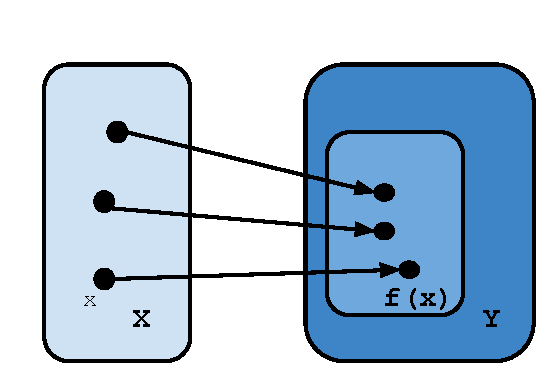
\includegraphics[width=0.5\linewidth]{figs/fn.pdf} 
  \caption{A transformation is only legal if
  the transformed input $x$ is in the set of valid inputs for the API function
  $f$, and the new outcome $y$ is in the set 
  of valid outcomes for $f$. For the network API, this means 
  that the outcome $y$ could have been observed 
  for $f(x)$ on a correct network.}
  \label{fig-fn}
\end{figure}

API calls can be invoked in an 
Affix component by an application or by another component.
The call may then be transformed and invoked in another component, 
or in the network stack of the host \ac{OS}.
Return values from API calls are transformed and propagated to the 
caller in the reverse direction.



\begin{figure}[htb]
  \centering
  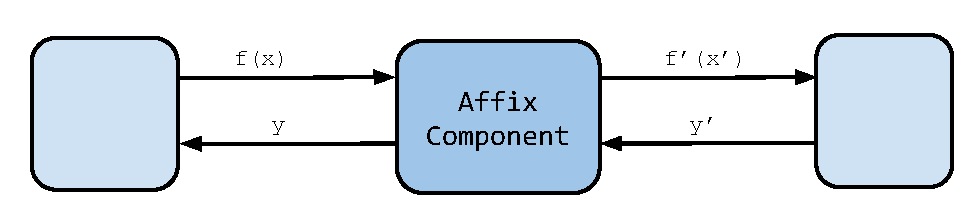
\includegraphics[width=\linewidth]{figs/component_wide.pdf} 
  \caption{An Affix component transforms a function and its input and invokes 
  another component, while returning transformed output
  to its caller. 
  }
  \label{fig-component}
\end{figure}



% Fraidy: I prefer to defer this to the implementation section
%
% The position of Affix components between the application and 
% the operating system's network stack 
% demands that they be compatible with 
% the socket API interface. This is true for both 
% the upwards (presenting a socket interface to the application or 
% Affix component above) 
% and the downwards direction (interfacing with the socket or 
% socket-like structure below it). 
% The Affix component is free in its design of internal workings as 
% long as it respects interface compatibility.

% In practice, interface compatibility requires that an Affix 
% component implements interfaces that match the different 
% groups of operations available on an actual socket, i.e. 
% address resolution (\texttt{getaddrinfo()}), 
% connection management (\texttt{listen()}, \texttt{connect()}, 
% \texttt{accept()}, etc.), 
% data flow (\texttt{send()}, \texttt{recv()} ...), 
% and possibly configuration (in the form of socket options).

% In addition to the interfaces required per the socket \ac{API}, 
% an Affix component must implement a number of Affix-specific 
% functions for instantiation and configuration, including 
% ones for combining multiple Affixes. We will discuss these 
% in an instant.


\subsubsection{Special components}
\label{special}

A particular API call is called \textit{transparent} for a component
if it  preserves interface semantics itself, without
requiring the application of another 
operation. That is, if the component transforms 
$y = f(x)$ into $y' = f'(x')$, and
$y'$ is also a valid output of $f(x)$, then $f(x)$
is transparent in this component. If every API call 
in a component has this property, then the entire component 
is transparent. For example, a \textit{RateLimit} service 
that performs traffic shaping
can be implemented in a transparent component.

In the socket API, the \texttt{send()}
 and \texttt{connect()} calls propagate data and associations, 
 respectively, while the \texttt{recv()} and \texttt{accept()}
 calls consume these.
If a propagating API function $f$ is not transparent for a component, 
then the component must also implement the consuming equivalent function 
$g$ such that the application of $f$ followed by $g$ 
preserves interface compatibility -- i.e., that it gives a 
result that could be observed on a correct network. 
\cappos{Assuming that a component must `mirror' itself... (see later comment
in 5.2)}
For example, if the \texttt{send()} call of a 
\textit{Compression} component 
compresses data before sending it over the network, 
the \texttt{recv()} call of the component should decompress 
received data before returning it to the application.


A component that transforms a propagating 
call into its consuming equivalent, and vice versa,
is called a \textit{mirroring} component. 
Mirroring components also reverse the direction 
of invocation on their output.
The network itself is modeled as a mirroring component, 
as it transforms API calls like \texttt{send()}  
into \texttt{recv()} calls. Figure~\ref{fig-mirroring}
shows how the network transforms a \texttt{send()}
call invoked on one side into a 
\texttt{recv} call on its other side.

\begin{figure}[htb]
  \centering
  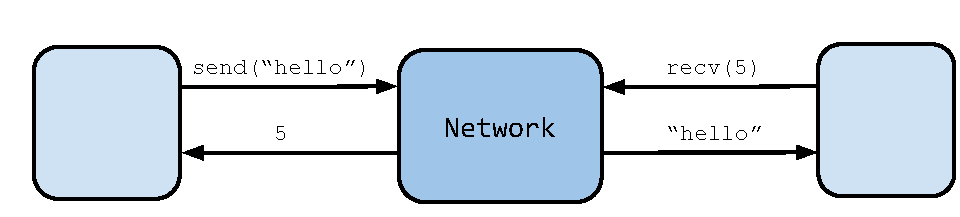
\includegraphics[width=\linewidth]{figs/network.pdf} 
  \caption{The network itself is modeled as a
  \textit{mirroring} component. It transforms calls 
  that propagate (e.g., \texttt{send()}) into 
  calls that consume (e.g., \texttt{recv()}) and 
  reverses the direction of invocation on its output. }
  \label{fig-mirroring}
\end{figure}


Other special components include \textit{manager}
components, which add or remove other components 
and links between components, and
\textit{branching} components, which may invoke 
a function in more than one next component.  
The \textit{Coordination} service discussed 
in detail in Section~\ref{subsec-services-coordination} is a manager, 
and a branching component is illustrated 
in Figure~\ref{fig-tree} (node $A$).


\subsection{Combining Affix components}
\label{subsec-arch-stack}

% \begin{figure}[htb!]
%   \centering
%   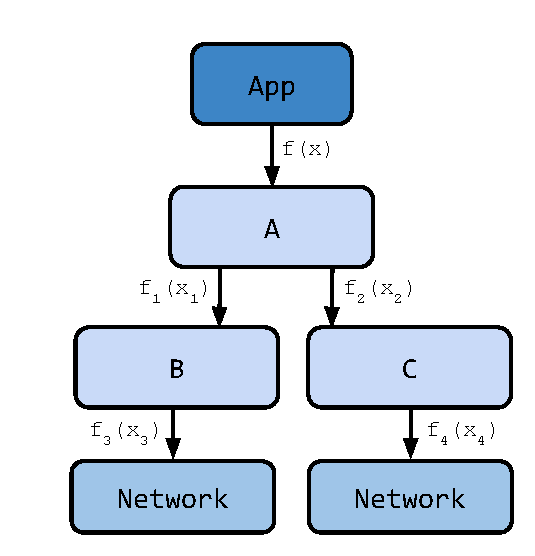
\includegraphics[width=0.7\linewidth]{figs/tree.pdf} 
%   \caption{The set of Affix components operating on one
%   socket form a rooted tree, with arcs showing the 
%   invocation relationship between components.}
%   \label{fig-tree}
% \end{figure}


% Validity of permutations doesn't mean every permutation is meaningful.
Affix components that act on a single socket
in an application
are organized as a rooted tree.
Every Affix component is represented as a 
node in the tree, with arcs showing that 
the source node may invoke calls in the destination node.
A sample tree is given
in Figure~\ref{fig-tree}.

When the application calls an 
API function, the call is handled first by the root node.
Each node in the tree may transform the call
and then one or more child nodes. A
terminal node calls the underlying network API, propagating 
the function call to the \ac{OS} network stack, which in turn 
passes data through the network. 


% Given interface compatibility towards both the next-higher and 
% lower layers means that an Affix component need not necessarily 
% call into the actual \ac{OS} socket, or be called by the 
% actual application from above. Rather, Affix components can be 
% situated on top of one another, a setup we refer to as an 
% \textit{Affix stack}. Through stacking, complex functionality 
% can be assembled from multiple simple Affix components, an approach 
% that follows good design practice -- it advertises reuse, and keeps 
% single Affix components light-weight.

% We required before that the composition of services in a 
% componentized networking framework must be dynamically modifiable 
% for it to achieve maximum impact. Each Affix component is therefore 
% aware that it might live in an Affix stack, and includes functionality 
% to modify the stack below it. Specifically, an Affix component can 
% add or remove other Affix components below it to adapt the stack's 
% capabilities to that of the remote side.



\subsection{Propagation of API calls}
\label{subsec-arch-flow}

When connected through the network (which, 
as described in Section~\ref{subsec-arch-stack}, is itself
modeled as a component), 
the Affix components through which data 
for a particular communication travels make up 
a graph. This graph includes the Affix 
tree at each endpoint, as well as those on relays 
or other middleboxes. 
Figure~\ref{fig-dataflow} shows an example of an Affix graph.

\begin{figure*}[htb]

  \centering
    \begin{tabular}{c c}  
    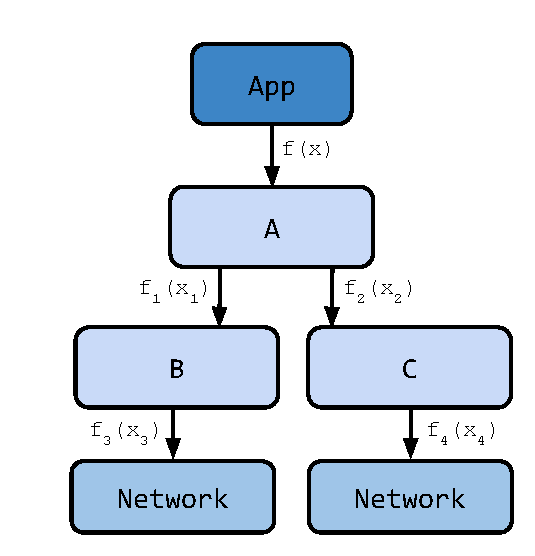
\includegraphics[width=0.35\linewidth]{figs/tree.pdf}  \hspace{.05cm} &
  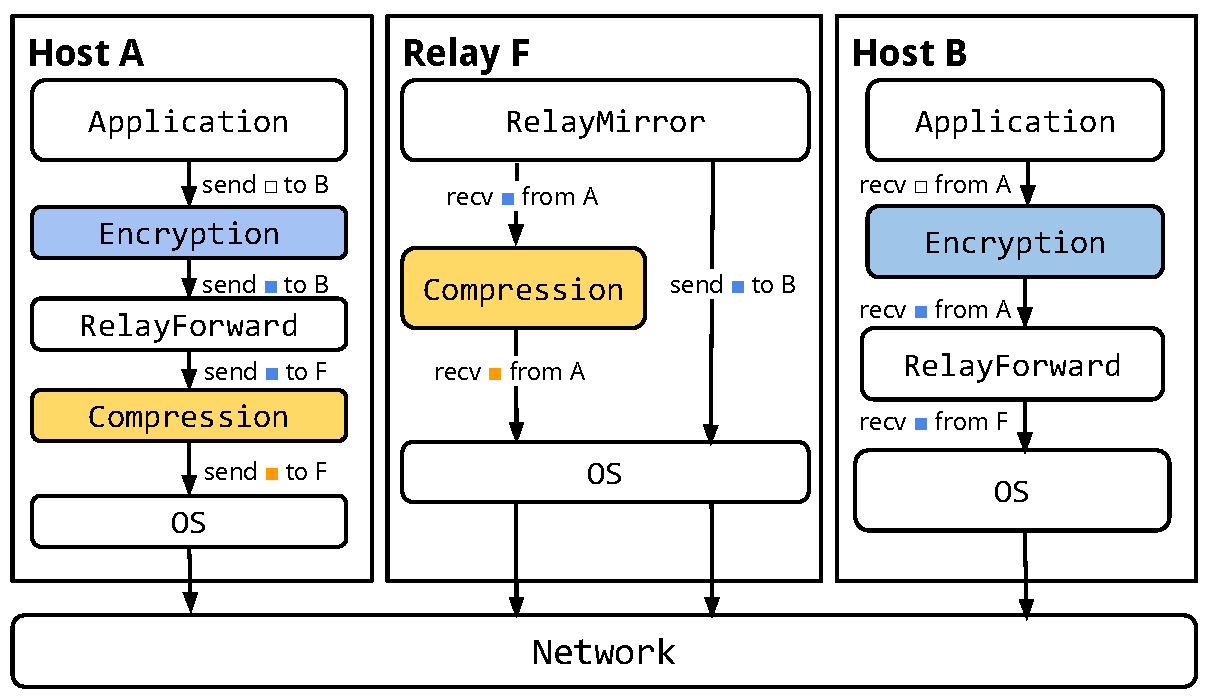
\includegraphics[width=0.6\linewidth]{figs/propagation.pdf}    \\
  \end{tabular}
  \caption{(left) The set of Affix components operating on one
socket form a rooted tree, with arcs showing the 
invocation relationship between components.}
\label{fig-tree}
\caption{(right) This figure shows how Affix components 
  intercept an API call, transform the data and endpoints 
  associated with the call, and propagate the call through 
  an Affix graph until it reaches its destination.}
\label{fig-dataflow}

\end{figure*}

%      \caption{This figure shows how Affix components 
%  intercept an API call, transform the data and endpoints 
%  associated with the call, and propagate the call through 
%  an Affix graph until it reaches its destination.}
%  \label{fig-dataflow}


%  \caption{This figure shows how Affix components 
%  intercept an API call, transform the data and endpoints 
%  associated with the call, and propagate the call through 
%  an Affix graph until it reaches its destination.}
%  \label{fig-tree}



In Figure~\ref{fig-dataflow}, an application on Host A
calls \texttt{send()} with some data to send and a destination
endpoint. This figure illustrates the requirements for 
a path through the Affix graph to satisfy
end-to-end interface compatibility:

\begin{itemize}
 \item Any non-transparent call must be followed by its mirror
 call.
 \item If a function $f$ that is not data transparent is called 
 before a function $f'$ that is also not data transparent, then 
 their mirror functions must occur in the reverse order: 
 $g'$ before $g$. 
\cappos{Stray thought: What if the order is fgf?   (I know the answer
and the reader will too, but we may get this comment from a reviewer.)}
\item Calls that transform the endpoint associated with a call
must be transparent end-to-end, i.e., their composition must 
satisfy the requirements for transparency described in 
Section~\ref{special}.
\end{itemize}


\subsection{Coordination Service}
\label{subsec-services-coordination}
\cappos{Make this more formal.   Leverage the formalisms to define
a calculus for communication in this domain...}

Most Affix services operate on network traffic to improve performance, 
but unlike standard library or other implementations 
of these services, they can be deployed in a democratic fashion. 
However, they do not themselves contribute to democratic deployment. 
In contrast, the function of the \emph{Coordination} service is to 
enable democratic deployment. 

The Coordination service identifies the Affix components used 
by an opposite side of a communication flow, then loads a matching 
set of Affix components on the local host.
This enables communication through any composition
of services without prior arrangement.
The Coordination service described in this section is 
the exemplar service included in the Affix implementation and 
deployed on the Seattle testbed; 
it is also possible to implement alternative coordination services
with equivalent functionality but different properties.


\iffalse

While some Affix components can be used by either side of a 
connection transparently, many components will 
require some level of client-server communication in order 
to work properly. The client and server
needs to balance the Affix stack against each other in order 
to ensure proper communication. Take
for example that the server is using both the CompressionAffix 
and the EncryptionAffix in order
to compress and encrypt it's communication. If a client wants 
to connect and communicate with the
server, than they must also use the proper CompressionAffix 
and EncryptionAffix in order to be able
to decrypt and uncompress the data before returning the data 
to the application layer. In order for
the client to find out that the server is using these two 
components, it needs to be able to communicate
and coordinate with each other to ensure both sides are 
using the same Affix stack.

The practicality of different approachs taken to coordinate 
Affix stack information between clients and servers 
will depend on several factors. Consider the following 
two approaches.  

Approach One: A special purpose Affix component is put in place at the bottom of the network stack. 
Whenever a packet is received this componen willt facillitate communications to ensure the correct 
Affix stack is put into place on both sides of the connection.

Approach Two: A sever decides what Affixes will be used, and advertises the result under an applicaiton 
specific identifier, and port number in a secure look up service.  When a client program wants to connect 
to a server a look up is performed to find out what Affixes should be put into place. 

The first approach had the bennifit of not requireing an outside service, or the overhead added 
by advertisements and look ups.  As long as connection establishement is not an issue coordination 
of Affix stacks in this manner is perferable.  The second approach is, however, the only viable one 
in many situations. Consider for instance that no direct connection can be established to a particular server.  
The server can impose a NatPunchAffix that accepts traffic through a publicly reachable forwarder, 
but the client must some how learn what Affix stack to use in order to connect.  
\fi


The Coordination service implemented in Affix is always placed at the root
of an Affix tree. It redefines \texttt{listen()} to call
\texttt{get\_advertisement\_string()}. This returns a serialized description 
(called an \emph{Affix string})
of all non-transparent services underneath itself in the Affix tree.
The address at which it would like to be reached and the Affix string
with which it can communicate are sent as a key-value pair to 
a public \emph{advertise service}. Finally, the service invokes \texttt{listen()}
in the Affix component beneath itself.

When the opposite host calls \texttt{connect()}, the Coordination service 
queries the advertise service to find the Affix string stored for the 
given destination address. It then constructs a matching Affix tree beneath itself.

\albert{Fraidy noted: ``What is interesting? notable? about this coordination service?''}

\cappos{I was thinking something similar.   I was also thinking another
way to spin this is as protocol / service negotiation...}


\iffalse
Thus we implemented the second approach by leveraging an advertise service in order to
build the CoordinationAffix component which allows the client to do a lookup and build the
Affix stack the server is using, even if the server is directly unreachable. The advertise
service we use consists of multiple servers that are available on public domains. The service
has a redundancy system in order to ensure the service is always available.

The CoordinationAffix on the server side usually lies at the top of the stack and has a view
of all the Affixes that are in the stack. The CoordinationAffix serializes the stack on the
server side and advertises the serialized string on the advertise service. The CoordinationAffix
on the client side does a lookup on the advertise service to retrieve the serialized form of the
Affix stack. The coordination component than deserializes the Affix stack string and builds
the new Affix stack on the client side before making any network calls. Note that the 
CoordinationAffix only serializes the non-transparent Affixes that need to exist on both
sides of communication in order for the two nodes to communicate properly. Examples of such
components are CompressionAffix, EncryptionAffix and NatPunchAffix. The CoordinationAffix
however does not advertise transparent Affixes, such as LoggingAffix, StatAffix and RateLimitAffix.
\fi




\subsection{Naming}
\label{subsec-implementation-discussion}

\cappos{Does this belong earlier?   It ties in well with the deployment
subsection...}

An important aspect of democratic deployability is the ability to support 
communication with legacy (non-Affix) clients and servers.   In other 
words, Affix itself should be democratically deployable.   %To support
%this, there are several important challenges.
%\cappos{We likely need to discuss naming before this...}
However, on the Internet, hosts are commonly identified by 
a DNS name.   The DNS name is then mapped to an IP address.
However neither of these serve as a unique identifier
for a communication endpoint, especially in the presence of NAT boxes.
If we ignore non-Affix applications for the moment, it would be possible
to simply have an Affix endpoint use a Affix ID
as a name in a global registry similar to DNS.   (For scalability reasons,
such a registry can be implemented as a distributed hash table.)
The client could look
up the ID and use the resulting information (such as the serialized 
Affix stack) to understand how to contact the server.   However, this only
will work when both the server and client support Affix.
\cappos{I need your help here.   This text is rough to say the least.}

Applications must work correctly with either a client or a server does not 
support Affix.   If a server does not support Affix but the client does support
Affix, then it is trivial for the client to simply contact the server
without Affix.
However, an unmodified legacy client 
must be able to communicate with an Affix server.   If a legacy client knows
the server's IP or hostname instead of its Affix ID, the client can connect
to the server.
%the client does not know how to connect to a server given an Affix ID.

However, in some cases a server is not directly by IP address (eg when
behind a NAT).
For legacy clients that use a hostname, it is possible to still support
Affix by overloading the existing name.  To do this, a service called 
Zenodotus maps every
Affix ID to a valid DNS name.   A client using a Zenodotus name
(ending in {\tt zenodotus.[anonymized].org}) and it is resolved to an
IP address where the client may contact the server. 
%For example, in Figure~XXX(a), a webserver wants to support compression
%for Affix clients while also supporting legacy clients.   Legacy
%clients will look up the webserver's DNS name and contact it on 1.2.3.4, port
%80.   However, Affix clients will lookup the Affix ID and find that the
%server supports compression on port 8000.   An Affix enabled client can take
%advantage of this support.
%
%Note that the Affix ID for a server need not refer to the host's IP address.
For example, in Figure~XXX, a server behind a NAT is contactable by 
providing the
relay's IP address to legacy clients.   In this example, Affix clients are 
able to connect to the server.   Additionally, clients that support
Affix will benefit from compression and encryption while communicating
over the relay.

%Given a portion of the address space to map names into (such as exists in 
%IPv6), Affix could also support legacy clients that use IP addresses
%instead of hostnames.
%\cappos{Is this too tangental?}



%A legacy client can use the DNS name
%to uniquely refer to the server.  Zenodotus will resolve this to
%an IP address that a legacy client can use to communicate with the server
%(Figure~XXX).   This 
%Affix components that are transparent to the client.
%XXX
%
%However, a server may have different services running on different ports.
%If the same hostname is used, then the same public relay must be used
%for all ports on the server.   This may be less than ideal because different
%applications / flows may want to relay through different systems.   To
%mitigate this, the XXX




\cappos{I'm intentionally dodging ports / protocols because I think it muddies
the water too much.}

\subsection{Deployment paths}
\label{subsec-deployment}
\cappos{Needs to be less implementation specific and more general...}

% Fraidy: I do not like this idea of an "uncooperative"
% application. I also want to focus more on "who" rather 
% than "where"

% There are two orthogonal concerns when deploying Affix with an 
% application: \textit{Cooperation} -- the application might or 
% might not actively expect and liaise with the Affix framework --, 
% and \textit{location} -- Affix components can be deployed at 
% different elements along the network path.

% A cooperative, i.e. Affix-aware, application includes Affix 
% functionality natively by using the  Affix libraries, so that 
% users will benefit without having to explicitly load Affix
% stacks on their own. An uncooperative application can be 
% forced to use Affixes either by relaying its traffic through 
% an Affix-aware \textit{proxy} application (on the same host, or 
% on a separate middlebox), 
% or by \textit{interposition} on its network library calls, 
% e.g. by setting the \texttt{LD\_PRELOAD} variable in Linux so that 
% Affix functions will be used before those of the same name in 
% the standard libraries. 
% Either way, program behavior is modified non-invasively, 
% and it can be configured system-wide 
% or used selectively on a per-application basis.


The Affix framework and core services may be installed as a 
Python package. Once installed, 
there are several methods available for using 
Affix, including:
\begin{itemize}
    \item \emph{Proxy}-based use. The Affix package includes a Python proxy,
which can load an abitrary Affix configuration. 
Traffic must be tunneled through the 
proxy for Affix functionality to be applied.
    \item \emph{Interposition}. The Affix library may interpose on network library calls 
(e.g., by setting the \texttt{LD\_PRELOAD} variable in Linux) so that 
its functions will be used before those of the same name in the standard libraries. 
    \item \emph{Native} integration within an application. A developer can 
choose to include Affix functionality natively in an application using the Python 
library.
\end{itemize}
The first two cases are suitable where the source code of an application 
is not available, where native integration is not practical, and/or when 
Affix is deployed by a non-programming end user.
In both proxy- and interposition-based use, 
program behavior is modified non-invasively, and it can be configured system-wide 
or used selectively on a per-application or per-socket basis.
\cappos{I thought ``How?'' when reading here.   Maybe describe a decider 
component in a sentence.}


% Albert: How about \multirow's and sub-figures?
\begin{figure*}[t]
  \centering
  \begin{tabular}{c c c c}  
  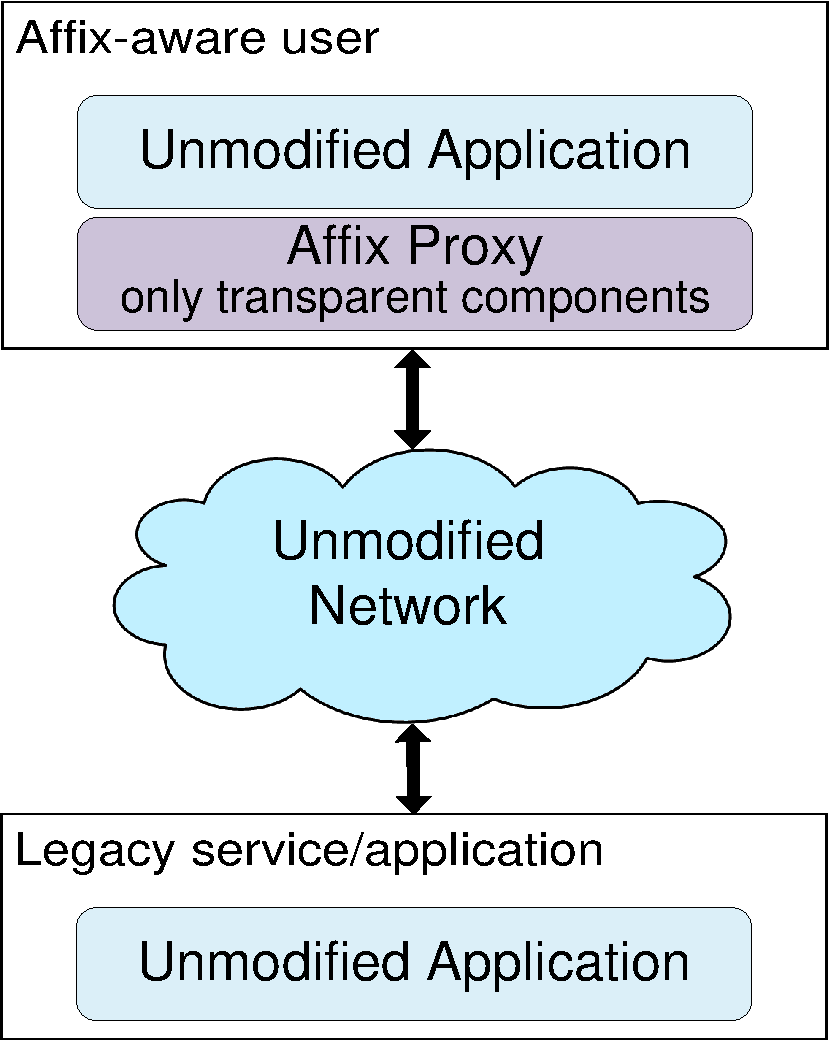
\includegraphics[height=4.75cm]{figs/dep3.pdf} \hspace{.05cm} &
  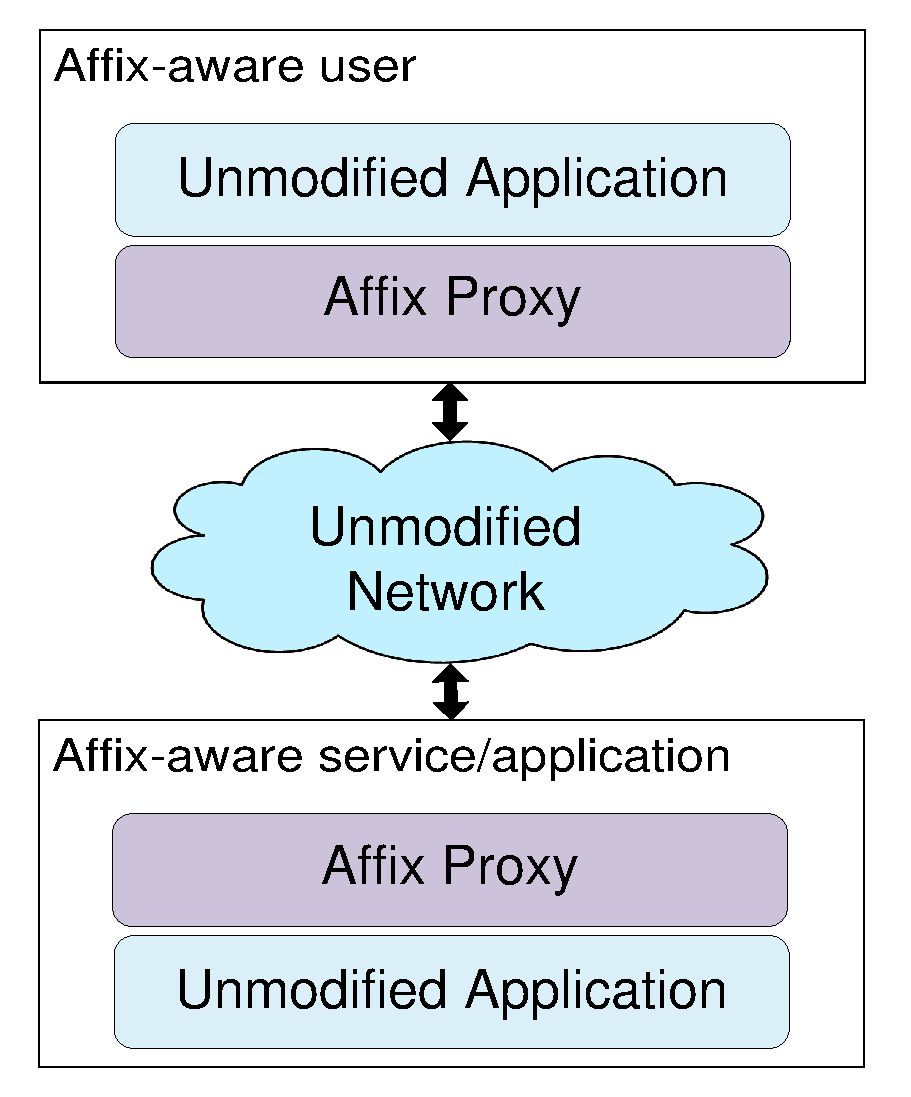
\includegraphics[height=4.75cm]{figs/dep2.pdf} \hspace{.05cm} &
  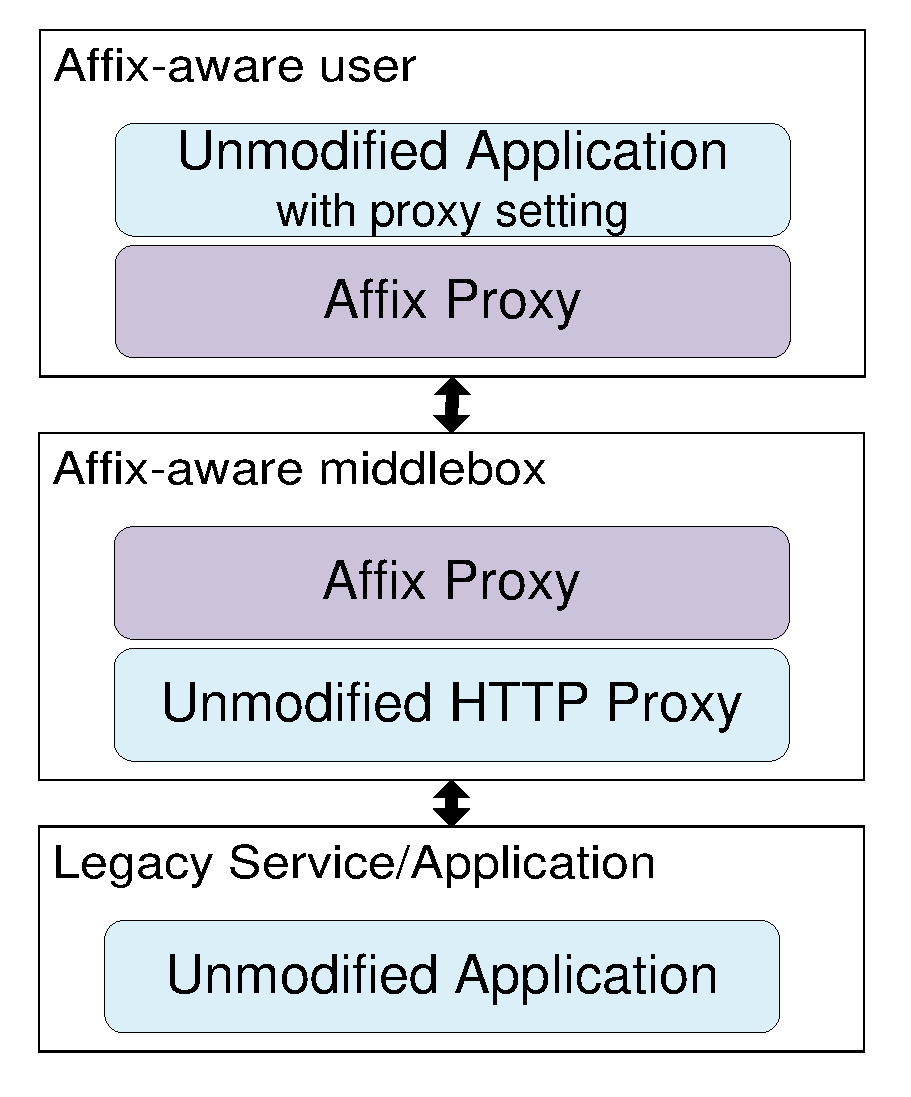
\includegraphics[height=4.75cm]{figs/dep1.pdf} \hspace{.05cm} &
  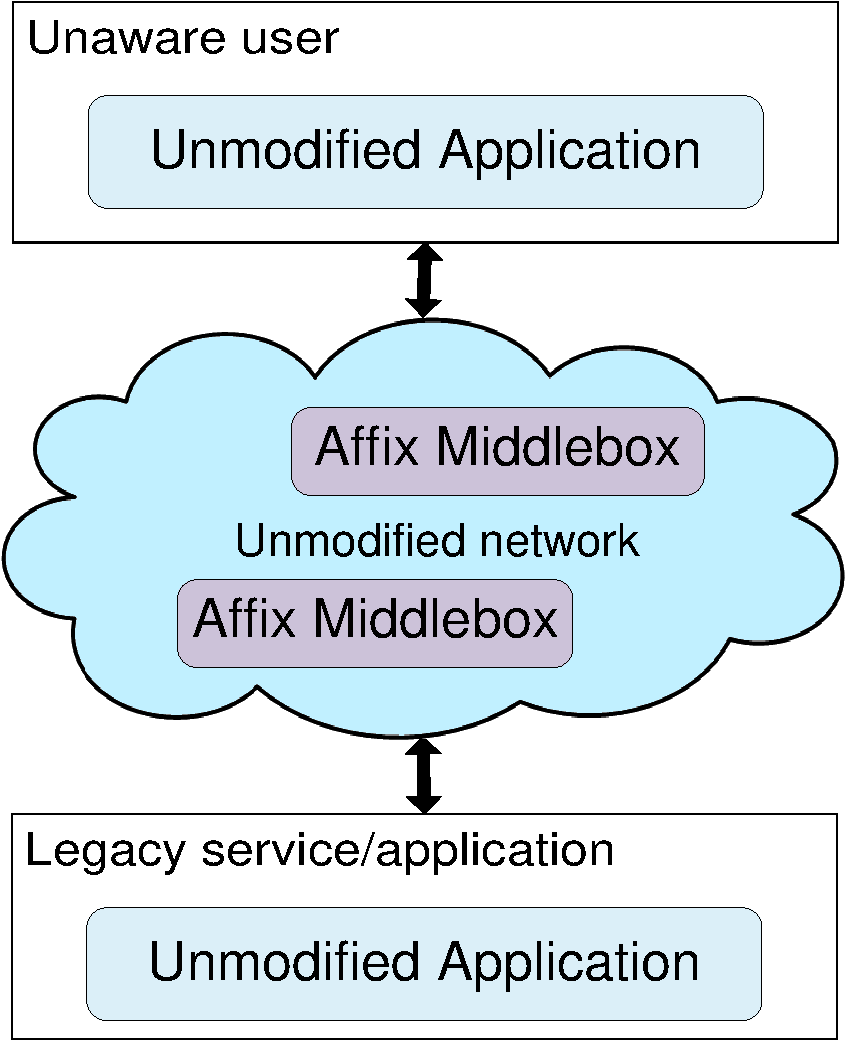
\includegraphics[height=4.75cm]{figs/dep4.pdf} \\
  (a) Only user is  \hspace{.05cm} & (b) User and service \hspace{.05cm} &  (c) User and middlebox \hspace{.05cm} &  (d) Only the core network \\
  Affix-aware  \hspace{.05cm} & are Affix-aware \hspace{.05cm} &  are Affix-aware \hspace{.05cm} &  is Affix-aware
\end{tabular}
  \caption{Affix supports various deployment paths for unmodified applications, depending on which parties are involved. Note that it is possible to use Affix if only the end user is 
  Affix-aware, as shown in Figure~\ref{affix-deployment}(a), 
  as well as when neither end user nor web service provider are Affix-aware, 
  as in Figure~\ref{affix-deployment}(d).   Applications co-located with
an Affix proxy may alternatively be changed to natively support Affix.}
  \label{affix-deployment}
\end{figure*}


Figure~\ref{affix-deployment} shows four possible deployment 
options available for use with unmodified applications
(i.e., the application developer is not a cooperating party). 
These deployment options are especially 
important in the context of democratic deployment, 
and several are unique to the Affix framework:

\begin{itemize}
    \item A user can run an Affix proxy to use transparent 
Affix components (such as rate limiting), and tunnel traffic from applications 
through the proxy, as in Figure~\ref{affix-deployment}(a),
    \item Users on two sides of a connection can run the 
proxy with double-sided Affix components (such as compression or encryption),
and tunnel traffic from applications through the proxy, as in Figure~\ref{affix-deployment}(b),
    \item A user can run the included Affix proxy to use double-sided and single-sided
Affix components, and direct traffic from applications to a proxy elsewhere on 
the Internet that offers Affix functionality, as in Figure~\ref{affix-deployment}(c)
    \item Traffic can be routed through an Affix stack without deploying 
    Affix on any end devices, by applying the interposition 
method on middlebox devices as in Figure~\ref{affix-deployment}(d).
%    \item An operating system can use the interposition method to 
%support Affix functionality with every application,
%    \item An application developer can use Affix components directly 
%within an application,
%    \item An advanced user or application developer can use Affix components 
%directly in a wrapper around an application.
\end{itemize}

